\chapter{Introduction} % Main chapter title

\label{Introduction} % For referencing the chapter elsewhere, use \ref{Chapter1}}

Complex system is a collection of a large number of units, they can interact with each other and because of the interaction some collective behaviour can emerge. The properties of the system can not be predicted from behaviour of one individual. 

Statistical physics attempt to describe behavior of large number interacting particles, atoms and molecules and macroscopies properties for example magnetisation is explained from interaction between particles. Also as complex system we can consider people i sociaty, population of fishes showing flocking pattern, traffic on the roads. 

\section{Complex networks}

The first mathematical problem solved using graph theory was $Konigsberg$, Kaliningrad in Russia, the problem of seven bridges. The city $Konigsberg$ in that time had seven bridges, that were connecting the parts of the city across the river and the island in the middle. The question was is it possible to find a walk that crosses all seven bridges only once. Representing the problem as a graph, Euler managed to simplify the problem, the parts of the land are represented as nodes while bridges between them are links. Crossing each bridge only once is possible if each part of the land has an even number of connections. Thus, in this case it was not possible, as each piece of land was connected with an odd number of bridges.

\begin{figure}[h!]
	\centering
	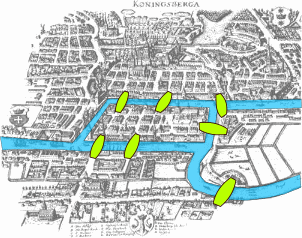
\includegraphics[width=0.3\linewidth]{Figures/Konigsberg_bridges.png} \hspace{2cm}
	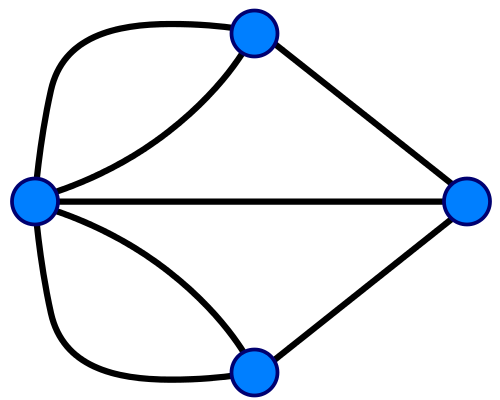
\includegraphics[width=0.3\linewidth]{Figures/Konigsberg_graph.png}
	\caption{The Kronigsber problem of seven bridges.}
	\label{fig:Krgraph}
\end{figure}

Despite the differences among complex systems, they can be represented in unique way, using graph theory. The real nature of the components is neglected, and we only represent the interaction among them. This approximation, allow us to treat equally social (graph of actors), biological (network of proteins) or even technological system (internet, traffic). In recent years complex network theory finds the application in different fields, and it's development is encored by availability of big data.

%Analyzing and Modeling Real-World Phenomena with Complex Networks: A Survey of Applications
%Characterization of Complex Networks: A Survey of measurements

\section{The structure of complex networks}

The complex system can be represented by complex network $G=(V, E)$, where the elements of system (atoms, proteins, people) map to set of $N$ nodes $V=\{1, 2, ...,N\}$. The interactions between elements map to $L$ links between nodes, $E = \{ e_1, e_2... e_L\}$. The \textbf{adjacency matrix} $\boldsymbol{A} = N \times N$ has value $1$ if there is connection between two nodes, otherwise it is $0$ \cite{boccaletti2006}. 

The network properties directly depend on the connectivity between nodes. In the case of regular networks, such as grids, each node has equal number of first neighbors. In general case, the networks have more complicated structure. Thus the important measure is network \textbf{degree} $k$. The degree of node $i$ gives the number of nodes attached to node $i$, $k_i = \sum_j A_{ij}$. The \textbf{degree distribution} $P(k)$ is probability that randomly chosen node has degree $k$. It can be calculated as fraction of $k$ degree nodes $N_k$, $p(k) = N_k/N$. The degree distribution in random network, where all nodes have the same connecting probability follows Poisson distribution $P(k)= \frac{(Np)^ke^{-Np}}{k!}$, where $k$ is mean degree distribution. In real networks degree distribution follows power law. Therefore, real networks have scale-free structure with emergence of the hubs \cite{newman2010}.

The \textbf{degree-degree correlations} in the network are measured by \textbf{assortativity}. If correlations are positive, networks are assortative; there is a tendency that connections exist between similar degree nodes. The negative correlations indicate that large degree nodes have preference to connect nodes with small degree; dissasortative networks. The average first neighbor degree $k_{nn}$ can be calculated as $k_{nn} = \sum_{k^{'}}k^{'}P(k^{'}|{k})$. The $P$ is conditional probability that an edge of degree $k$ points to node with degree $k$. The norm is $\sum_{k^{'}}P(k^{'}|k)=1$, and detailed balance conditions \cite{boccaletti2006},  $kP(k^{'}|k)P(k) = k^{'}P(k|k^{'})P(k^{'})$ \cite{boccaletti2006}. If the node degrees are uncorrelated, $k_{nn}$ does not depend on the degree, otherwise increasing/decreasing function indicates on positive/negative correlations in the network.

The Newman defined the assortativity index $r$ in slightly different way:
$r = \sum_{kl}kl(e_{kl} - q_lq_k) / \sigma_q^2$, where $e_{kl}$ is the probability that randomly selected link connect nodes with degrees $k$ and $l$, $q_k$ is probability that randomly choosen node is connected to node $k$ and equals $q_k = kp_k / \langle k \rangle$, while $\sigma_q$ is varience of the distribution $q_k$. 

The \textbf{clustering coefficient} is measure that describe the structure of neighborhood. In networks exist tendency of forming triangles or clusters. This is common in friendship networks where two friends of one pearson have high probability to be friends. The clustering can be measured by computing the number of links between neighbours of one node, $c_i=2e_i/(k_i(k_i-1))$. Averaging it over all nodes in the networks we can calculate mean clustering coefficient. It ranges from  $\langle c \rangle = 0$ where connections between neighbouring nodes do not exist, network has structure of three. On the other hand $\langle c \rangle = 1$ indicates fully connected network. 

Real world networks share similar properties. Mean distance between nodes is small and it is much smaller than number of nodes in the network $l << N$, this property is called small world phenomena. This cause the fast spread of information or even diseases in the complex systems. In small world networks number of vertices grow exponentially with distance, thus $l$ increase as $log(n)$ or slower. Logarithmic scaling can be proved from various network models, also it is observed in real world complex systems. Clustering coefficient in the real world networks is usually high. Real world networks have one important feature; power-law degree distribution; such networks are called scale-free networks.

\section{The dynamics of complex networks}

\subsection{The random graph model }

The random graph moddel was introduced by Erdos and Renyi in 1959. This model has $N$ disconnected nodes. With probability $p$ each pair of nodes can be connected.  The network is characterized only by number od nodes and links, $G(n, p)$. 

As this process is stochastic, the network with same parameters n and p, does not have to be same structure, so it is necessary to consider the ensemble of networks. Then the mean number of links depends on the model parameters:
$\langle m \rangle = n(n-1)p / 2$. The expected value of node degree can be predicted as $\langle k \rangle = (n-1)p$.
The probability $p$ is defined as density of the network. 
The probability $p(k)$ follows the binomial distribution of the form:

$p(k) = p^k(1-p)^{n-1-k}$. For large values of $n$, this becomes $p(k) = e^{-k}k^{-k} / k!$, which is Poisson distribution. 

In the case of a large random networks, the average path length is given as $l = \frac{ln n - \gamma}{ln(pn)} + \frac{1}{2}$. This means that random graph has a very small average path length. This is characteristic of many large networks. 

The clustering coefficient $C=p$, so for sparse ER graphs the clustering is very small, much smaller than in real world networks.

Increasing the probability $p$, the giant component may appear. This is sub-graph whose size is proportional to the size of the network. Such change in the network is phase-transition and it is important as small change in the probability p leads to fundamental change in the system properties. There are two limits of this model, when $p=0$, network is disconnected. If $p=1$, then network is fully connected, and giant component is with size $O(1)$.  This phenomena is related to percolation phase transition. On the threshold $p_c$, the component whose size is proportional to $n^{2/3}$ emerges. Average path length between two nodes, at critical point is proportional to the $ln N$. The small, logarithmic distance is the origin of the "small-world" phenomena. 

The interesting behavior of this model is that, with increasing p nodes tend to organise in giant component. The subcritical , $k <1$ where all components are dimple and small. The size of larges component is $s=O(ln n)$. In critical regime $k=1$, the size of largest component is $s=O(n^{2/3})$. Supercritical $k>1$, where the probability of having giant component is 1.  


\subsection{Small world networks}

In the 1999. Watts and Strogatz introduces "small-world" model. This model can generate the networks with small diameter and high clustering coefficient. Their idea is to start from grid like network, where all nodes have same number of neighbors, like ring-lattice or hexagonal lattice, where each node is connected to k nearest neighbors. Such network has high clustering coefficient, as any pair of consecutive neighbors are connected forming a triangles, while in contrast the network has high average shortest path, as nodes on the oposite sides of the lattice are not connected. The goal of this model is to connect distant nodes and reduce the average path lenght in the network. This can be simply done by randomly rewiring nodes in the network, with probability $p$. Model interpolates between regular network $p=0$ and random graph $p=1$, and for some critical probability we can achieve small world networks. 

%TODO
% mozda dodati sliku ovog moddela

The average shortest-path length from the model is close to that of an equivalent network, and much lower than that of the lattice. The clustering coefficent from the model is still close to that one in the lattice and much larger than in random network. 

The degree distribution of this model obviously is not power-law. In regular network, all nodes have equal degree, while in random networks degree distribution becomes Poisson. 

\subsection{Barabasi-Albert model}

The random network model differs from real networks in the two characteristics, growth and preferential attachment. In static models, number of nodes is fixed, while in growing models we try to simulate the continuous change in the system. More important ingredient, are linking rules. In real networks, new nodes tend to link to more connected nodes.

This model is defined as follows, we start from $m_0$ nodes, randomly connected, and at each timestep we add new node with m links that will connect to $m$ nodes already present in the network.  The probability that new node connects to node $i$ depends on node degree $k_i$ as

\begin{equation}
P(k_i) = \frac{k_i}{\sum_jk_j} 
\end{equation} 

New node can connect to any node in the network, however nodes with larger degree have higher probability to link new nodes. After time $t$ the model generates network with $N=t+m_0$ nodes and $m_0+mt$ links. Degree distribution is power-law with exponent $\gamma=3$. As network grows nodes with larger degree becomes bigger, so we end up with few nodes with many links, called hubs. Two simple mechanisms are responsible for emergence of scale-free networks. 

 \textit{degree distribution}
 
To understand the emergence of scale-free properties we need to analyze the evolution of degree distribution. The rate at which an existing node get new links as result of new nodes connecting to it is

\begin{equation}
\frac{dk_i}{dt} = mP(k_i) = m\frac{k_i}{\sum_jk_j}
\end{equation}

each new node arrives with m links. The sum is $2mt - m$ so the equation for large t becomes:

\begin{equation}
\frac{dk_i}{k_i} = \frac{1}{2}\frac{dt}{t}
\end{equation}

solving this equation we get that degree of node in time step t is $k_i(t)=m(\frac{t}{t_i})^\beta$, where $\beta=1/2$. 

We note that degree of each node increase following power-law; the growth in degrees is sub linear, as each new node has more nodes to link than previous. The eirlier node $i$, the higher is its degree. Hubs are large as they arrived early in the network. 

In summary, the analytical calculations predict that the Barabási-Al-
bert model generates a scale-free network with degree exponent 3. The degree exponent is independent of the m and m 0 parameters. The degree distribution is stationary explaining how different systems have similar structural properties. 

In summary, the absence of preferential attachment leads to a growing network with a stationary but exponential degree distribution. In contrast the absence of growth leads to the loss of stationarity, forcing the network to converge to a complete graph. This failure of Models A and B to reproduce the empirically observed scale-free distribution indicates that growth and
preferential attachment are simultaneously needed for the emergence of the scale-free property.

In the past decade we witnessed the emergence of two philosophically different answers. The first one views preferential attachment as the interplay between random events and some structural property in the network. The second assumes that each new node or link balances conflicting needs. 

The BA model postulates the presence of preferential attachment. Yet, we can build models that generate scale free networks without preferential attachment. The link selection model offers the simplest mechanism that generates a scale-free network. At each time step we add new nodes to the network, we select link at random and connect the new node to one of the two nodes at the end. The higher is degree of the node, the higher is chance that node is located at the end of chosen link. The more k-degree nodes are there, the more likely is that k node is at the end of chosen link. Probability that node at the end of randomly choosen link has degree k is $q_k = Ckp_k$. The fact that bias is linear with k indicates that the link selection model builds scale-free networks. 
Copying model can also generate scale-free networks. In each time step a new node is added to the network. To decide where it connects we randomly select node u. Then with probability $p$ new node links to $u$, otherwise with probability $1-p$ we randomly choose an outgoing link of node $u$ and link the new node to its target. The likelihood that new node connects to degree-k node is $P(k)=\frac{p}{N} + \frac{1-p}{2L}k$, the second part is equivalent in selecting a node to randomly selected link. The popularity of the copying model lies in its relevance in real systems. It is common in social networks, citation networks or even protein interactions. 
in optimization, when new nodes balance conflicting criteria as they decide where to connect

\textit{diameter}
The network diameter, represents the maximum distance in the BA model, $d \sim \frac{lnN}{lnlnN}$. The diameter grows slower than $lnN$, making the distances in BA model smaller than in random graph. The difference is found for large N. 
\textit{clustering}
The clustering coefficient of the BA model follows $C \sim \frac{ln N^2}{N}$. It is different from clustering found in random networks, and BA networks are in general more clustered. 

\subsection{Nonlinear BA model}

In summary, nonlinear preferential attachment changes the degree
distribution, either limiting the size of the hubs $(\alpha < 1)$, or leading to su-
per-hubs ($\alpha > 1$, ). Consequently, $P(k)$ needs to depend strictly lin-
early on the degrees for the resulting network to have a pure power law p k .
While in many systems we do observe such a linear dependence, in others,
like the scientific collaboration network and the actor network, preferen-
tial attachment is sublinear. This nonlinear $P(k)$ is one reason the degree
distribution of real networks deviates from a pure power-law. Hence for
systems with sublinear  the stretched exponential (5.23) should offer a
better fit to the degree distribution.


In real systems preferential attachment can be more influenced by the age of the node. If parameter alpha is negative, ageing effect overcomes the role of preferential attachment, and scale-free properties are lost. For large negative alpha, the network turns into the chain, where the youngest nodes are the most attractive. On the other hand for a positive alpha, new nodes will link to older nodes. Positive alpha makes the network more heterogeneous, and scale-free nature still exist but exponent gamma is different from 3.  for the high alpha all nodes will tend to connect to oldest node. 

In the general ageing model, we have linking rules where rules connecting probability depends on both of node degree and age difference between new and old node.  With parameters alpha and beta we can control the structure of generated networks. I already talked about some limits of the general model. We saw that for specific parameters there are SF networks, BA model, if we move from that point SF behaviour with power-law with exponent 3 is lost. And other classes of networks can appear. In general, model, when alpha and beta are both positive, rich get richer phenomena is more promoted. On the other hand, the region where beta is positive and alpha negative can be interesting, because SF networks can appear only along the critical line. 

In growing network models is considered that at each time step one node is added to the network. The remaining question is if there is any change if network growth is not linear anymore and how does it influence the structure of obtained networks.  In this work, we use numerical simulations to explore the case when $M(t)$ is a correlated time-varying function and study how these properties influence the structure of generated networks for different values of parameter $-\infty<\alpha\leq-1$ and $\beta\geq1$ and constant $L$.

\section{ Network structures}
\subsection{Bipartite networks}

A bipartite network has two partitions, $U$ and $V$. The nodes in the same partition are not connected while links exist only between nodes of a different kind. Bipartite networks represent the membership of people or items in groups. For example, we can define the network of actors as a bipartite graph. In one partition are actors and in other movies. There are no edges between actors or movies, but the actor is connected to the film if it plays in that movie. Another example is a recommender network, such as a network of people and items they like. 

The equivalent representation of bipartite network is incidence matrix $B$. If $n$ is number of people and $g$ number of groups, this matrix is $g x n$, having elements $B_{ij}$ 1 if persoon i belongs to group j. 

Even bipartite networks give realistic representation of the system, there is often need to analyze the single type of nodes.  From a bipartite network, we can generate two projections. The first one connects nodes partition $V$ if they point to node $u$. Similarly, we can project the network on U partition, connecting $u$ nodes. The one mode projection between actors and movies onto actors is undirected network of actors. Actors are connected if they appear in the same movie. We can also create one-mode projection onto movies, where two movies are connected if they share the same actor.  

The projections are useful in some manner, but they also lose some important information, for example how many groups nodes share in common. This information can be propagated adding the weight to the edges, equal to the number of common groups.

The product $B_{ki}$ and $B_{kj}$ is 1 if $i$ and $j$ belong to the same group $k$. Thus the total number of groups to which nodes $i$ and $j$ belong is 

$P_{ij} = \sum_{k=1}^g B_{ki}B_{kj} = \sum_{k=1}^g B_{ik}^TB_{kj}$. The matrix $P$ is matrix of one-mode projection. The diagonal elements are non-zero, and represent the number of groups node $i$ belongs to.  To derive the weighted adjacency matrix, the diagonal elements are set to 0. The adjacency matrix of unweighted projection, each non-zero element needs to be replaced with $1$. 

\subsection{Core-periphery networks}

Core-periphery structure describes a network whose nodes are divided into two community, densely connected core and less connected periphery. If we consider the average probabilities of edges within each group as $p_{11}$ and $p_{22}$, and between groups $p_{12}$, instead of traditionaly assortative or dissasortative structure we can define core-periphery structure $p_{11}> p_{12} > p_{22}$. In the principle core-periphery structure does not have to be limited to only two groups, and we can define layered, onion, structure. The network can have more cores, that are not directly connected to each other. 

The simple method for finding core-periphery structure is to assume that nodes in core have higher degree in the core than in the periphery. Another simple method is to construct k-cores. K core is group of nodes that each has connection to at least k other members of the group. K-cores form a nested set, and become denser with higher k. The core-periphery structure can be detected optimizing the measure similar to modularity, as defined by Borgatti and Everett. Their goal is to find the division that minimizes the number of edges in the periphery. So they define the score function that is equal to number of edges in the periphery minus the expected number of such edges placed at random. $\rho = \frac{1}{2}\sum_{ij}(A_{ij}-p)g_ig_j$. They used genetic algorithm to minimize this function. 

The another way to detect core-periphery structure is to use the inference method based on fits to a stochastic block model. In this method we fit observed network to a block model with two groups, such that edge-probabilities have form $p_{11}> p_{12} > p_{22}$. The only downside of this model is that method is going to find the structure that optimize likelihood, and we can not say weather it is core-periphery or community structure. 

\subsection{Communities}

Thus the ability to find groups or clusters in a network can be a useful tool for revealing structure and organization within networks at a scale larger than that of a single node or a
few nodes. The occurrence of groups or communities is not limited to social networks.
Clusters of nodes in a web network, for instance, might indicate groups of
related web pages. Clusters of nodes in a metabolic network might indicate
functional units within the network. The ability to find groups also has another practical application: it allows
us to take a large network and break it apart into smaller subsets that can be
studied separately. The network in Fig. 14.1 is quite small, but others may be
much larger, millions of nodes or more, making their analysis and interpreta-
tion challenging. Breaking such networks into their component clusters is a
useful technique for reducing them to a manageable size. One example of this
approach is in network visualization. A network with a million or more nodes
can rarely be visualized in its entirety, even with the aid of good visualization
software. Such networks are simply too big to be represented usefully on the
screen or on paper. If the nodes of the network divide naturally into groups,
however, then we can make a simpler but still useful picture by representing
each group as a single node and the connections between groups as edges.
An example is shown in Fig. 14.2. This simplified representation allows us to
see the large-scale structure of the network without getting bogged down in
the details of the individual nodes. If one wanted to see the individual nodes,
one could then “zoom in” to a single group and look at its internal makeup. The problem of finding groups of nodes in networks is called community
detection. Simple though it is to describe, community detection turns out to be
a challenging task, but a number of methods have been developed that return
good results in practical situations.

\subsection{Stochastic block model}
The network or graph is the structure of nodes and edges, where each edge connects two nodes. Nodes can be organized into groups, called communities. Identifying these hidden blocks can lead to interesting insights into the network. However, the community detection problem does not give a precise definition of what a community is. As a consequence, many approaches try to recover such structural patterns in the network \cite{martin}.

A common definition of a community is that it is densely connected subgraph \cite{userguide}. We can find these subgraphs by optimizing an objective function, such as modularity function. It measures the difference in the number of edges between the given network and the network with the same number of nodes but randomly connected. In this approach, we try to maximize the density of connections inside a group by focusing more on assortative\footnote{Networks where nodes tend to connect with other nodes of a similar degree. Edges are more likely inside blocks than out of them.} group structures. 

Another type of networks is the bipartite network that has two disjoint sets of nodes. The edges exist only between nodes from different sets. Networks of this class can appear in real-world data, such as users-movies preference, collaboration network for scientists and papers, etc. Application of density-based approach requires to first project bipartite network to one of its partitions and then find communities in that projection. With this, some information is lost. On the other hand, the method that is directly applicable to bipartite networks is Stochastic Block model, from which the models considered in this paper are derived.

Stochastic block model (SBM) is based on connection probabilities between nodes. It is a generative model which includes existence of communities. Parameters that describe SBM for network G with N nodes are:

\begin{itemize}
	\item k: number of groups
	\item group assignment vector, g: $g_i \in\{1,2..k\}$, gives the group index of node $i$.
	\item SBM matrix, $p_{k \times k}$, whose elements $p_{ij}$ are the probabilities that edges between groups $g_i$ and $g_j$ exist.
\end{itemize}

Note that nodes within one group have the same connection probabilities.

SBM can generate and describe different types of network structures. Figure \ref{fig:SBM} \cite{userguide} shows how the model matrix corresponds to resulting networks with two communities. First, for the assortative network (\ref{fig:SBM} a), diagonal elements of the matrix have higher probabilities. This indicates dense connections inside the group, just like in classic community structures. In disassortative structure, (\ref{fig:SBM} b), more connections exist between two partitions than inside them, i.e. off-diagonal elements have higher probabilities. Bipartite networks can be represented like this. 

Figure (\ref{fig:SBM} c) shows how the model represents core-periphery networks. Nodes of one block (core) are well connected with itself and with other partition (periphery). From the last case, we can note that SBM with one group is the Erdos Renyi random graph (\ref{fig:SBM} d) because all probabilities inside and between groups are equal.

The benefit of this model is that we can generate many networks with similar group structure. The model can fit real data, which results in finding network communities. For the given network $G$ and number of groups $k$, the best nodes partition $g$ is found by maximizing the likelihood function. Beside inferring communities, SBM has application in prediction of missing links. This simply formulated model has many variants, motivated by specific properties of real data. For example, for networks which are degree heterogeneous, there is degree corrected SBM. In some social networks, users can belong to more than one group, and this can be modelled with mixed membership SBM. Other extensions include application to bipartite, weighted network, hierarchical model, etc. Also, several algorithms for optimization of likelihood function are proposed. The overview of these versions and methods are given in \cite{comparison}. In this paper, we will focus on Single and Mixed Membership SBM applied on bipartite networks.  
\begin{figure}
	\centering
	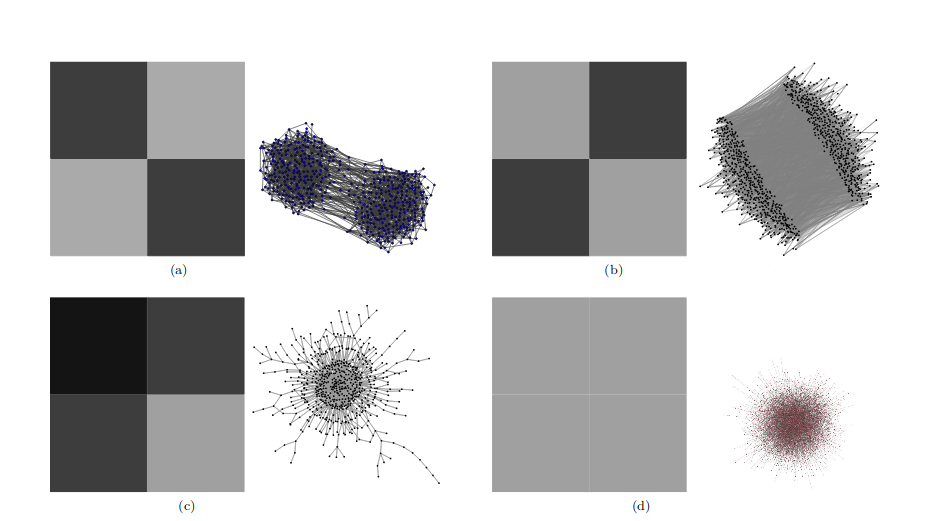
\includegraphics[width=0.7\textwidth]{Figures/structures.png}
	\caption{Stochastic Block model for different networks structures. (a) assortative. (b) dissortative. (c) core-periphery. (d) Erdos Renyi random graph.}
	\label{fig:SBM}
\end{figure}


\section{Graph isomorphism}

Weisfeiler-Lehman Test

\section{Distributions}

\subsection{power-law}
Power-law distributions characterize many social and biological systems. Power-law distributions are also easy to generate. 

the distributions: basic definitions and properties

The nonnegative random variable X is said to have a power law distribution if 
\begin{equation}
Pr[X>x] \sim c x ^{-\alpha}
\end{equation}

for constants $c>0$ and $\alpha >0$. In power-law distribution asymptotically the tails fall according to power $\alpha$. Such distribution leads to much havier tails than other common models, as exponential distribution. 

One specific power-law distribution is Pareto distribution which satisfies 

\begin{equation}
	Pr[X>x] = \frac{x}{k} ^{-\alpha}
\end{equation}

for some $\alpha>0$ and $k>0$. The Pareto requires $X>k$. The density function of Pareto distribution is $f(x)=\alpha k^\alpha x^{-\alpha-1}$. For power law distribution $\alpha$ is in the range $0 < \alpha < 2$, in which case X has infinite variance, if alpha <1 X has infinite mean.

if X has power law distribution, then a in log-log plot $Pr(x)$ will behave as straight line. For the specific case of Pareto distribution, the behaviour is exactly linear as $ln (Pr(x)) = -\alpha (lnx -ln k) $. Similarly the density function is also straight line. $ln(f(x)) = (-\alpha - 1) ln (x) + \alpha ln (k) + ln(a)$

\subsection{log-normal}
Many measurments in the nature show a more or less skewed distribution. They are common when mean values are low, variances are large and values can not be negative as example in distribution of minearal resources in the Eart. Such skewed distributions often closely fit to log-normal distribution. 

What is the difference between normal and lognormal variability? A major difference is that effect can be additive or multiplicative, leading to normal or lognormal distribution. Basic principles of additive and multiplicative effects can be easily demonstrated with the help od two dices. Adding the two numbers, which is the principle of the most games, leads to values from 2 to 12 with mean of 7, and simetrical frequency distribution. Multiplying the two numbers, leads to values from 1 to 36 with highly skewed distribution. Although these examples are not normal or lognormal they give us clear difference how different distributions can emerge. 

Log-normal distributions are usually characterized in the term of the log-transformed variable, using as parameters the expected value, or the mean, and the standard deviation. This characerization can be advantageous as by definition log-normal distributions are simetrical at the log level. 

The basic properties of the lognormal distributions

Random variable $X$ if $log(X)$ is normally distributed., if $Y=ln X$ has normal Gaussian distribution.  

Only positive values are possible for the variable and distribution is skewed. Two parameters are needed to specify lognormal distribution. Traditionaly the mean $\mu$ and standard deviation $\sigma$ or the variance of the $\sigma^2$ of $log(X)$ are used. However there are clear advantages of using transformed data, $\mu^{*} = e^{\mu}$, $\sigma^{*}= e ^{\sigma}$. The median of this lognormal distribution is $med(X)=\mu^{*}=e^{\mu}$, since $\mu$ is median of the $log(X)$.

\begin{equation}
f(x) = \frac{1}{x \sigma \sqrt{2\pi}}exp(-\frac{1}{2\sigma^2}(log(x)-\mu)^2)
\end{equation}

The mean is $exp(\mu + \sigma /2)$ and variance is $(exp(\sigma^2)-1)exp(2\mu+\sigma^2)$. 

Estimation: The asymptotically most efficient (maximum likelihood) estimators are 
\begin{equation}
x* = exp (\frac{1}{n}\sum_{i=1}^n log(x_i)) = (\prod_{i=1}^nx_i)^{\frac{1}{n}}
\end{equation}

\begin{equation}
s* = exp([\frac{1}{n-1}\sum[log(\frac{x_i}{x*})]^2]^{\frac{1}{2}})
\end{equation}


The lognormal distribution is skewed with mean $e^{\mu + \frac{1}{2}\sigma^2}$, median $e^\mu$ and mode $e^{\mu - \sigma^2 }$. It has finite mean and variance, in contrast to the power-law distribution.  

Despite it has finite moments, the lognormal distribution can be similar to power-law. If $X$ has a lognormal distribution then loglog plot of density function can apear as straight line for a large portion of a body of distribution. If the variance is large, the distribution may appear linear on log-log plot for several orders of magnitude. The variance of the corresponding normal distribution is large, the distribution may appear linear on a log-log plot. To see this we can check the logarithm of density function. 
If $\sigma$ is large then the quadratic term will be small for large range of x values, so the logarithm of the density function will appear almost linear for large range of values. 
Recall that normal distribution have property that the sum of two independent normal variables is normal variable. It follows that product of two lognormaly distributed random variables also has a lognormal distribution. 

\section{Scale-free networks}

The study of scale ivariance has a long tradition. Among the fields where this property was analysed were the theory of critical phenomena, percolations and fractal geometry. One of the first examples considered eas the price fluctuations  of cotton in commodities market (Mandelbort, 1963). The future price can not be obtained with arbitary precision from past series., still this series have some form of regularity. The curves for daily, weakly and montly price fluctuations are statistically similar. The fact that some features are found at different time scales is typical sign of fractal behaviour. Similarly in the case of coastline lenght we find fractal behavior. If we try to measure the total lenght, the real shape is so complicated that we always miss some part. 

Fractal behaviour might refer to different properties. In some systems scale-free structure is in shape. In this class the fractal shape can be robust, as in the case of branched patterns or electric breakdown. We say robust because these phenomena happen for varaity of external conditions. In the same class we have other systems that are more fragile, in the sense that they arise after precise tuning of some physical quantity. This is in the case of percolations and critical phenomena. Scale-free invariance may be related with dynamics or evolution of the system. The time activity of the system may display self-similar behaviour. The only sign of fractal behaviour is the mathematical form, power-law fluctuations of the time-series. 

The self-similarity can be present in the way the different parts of a system interact with each other. This is the case with self-similar graphs and the power-law scaling appers in the distribution of topological quantities like the number of interactions per part  of the system. These phenomena are fractals in the topology. 

\section{Scale-invariance and power laws}

The mathematical form of self similarity is represented by powe-laws. Whenever the function $y = f(x)$ can be represented as a constant to the power of x. The physical example is elastic force, the gravitational and electrostatic force. In the case of fractals, their geometry can be identified by considering the numbe of boxes $N(\epsilon)$, of linear size $1/\epsilon$. $N(\epsilon) = \epsilon ^{-D}$, where D is called fractal dimension. D can also be defined using mass relation $M = L^ D$.

Scale invariance is not restrected to geometry, but also appears in dynamical systems. In this case we have power-law distribution for different physical quantities. For example the evolution of some systems (sanspiles, number of species in the ecosystem) proceeds  with series of causally connected events whose size s is distributed as power-law. $P(s) s^{-\tau}$.

\subsection{plotting a power-law}

if we plot the data on double logarithmic scale, we should obtain a straight line. $y = x^{\alpha}$, $ln(y) = \alpha ln(x)$. The tail of the distributon is very noisy, and it is general feature of many experiments. To avoid the fluctuations in the tail it is common to use "binning" or cumulative distribution. 

In this method the noise reduction is done by deviding the $x$ axis into bins, and averaging the data within each bin. As an example we can take the frequency of numbers between numbers $1$ and $10$. Let assume that bin is $10$ units wide, we can represent all data in one point $b$, with $xb$ given by average of the bin extremes and $yb$ given by the avarage value of $ys$. If the bin size is constant for large values of $x$ the density of bins becomes very large as well. 

In the case of powerlaws it is usufull to use logarithmic binning. For example take the size of the first bin to be 2, and the others are power of 2. $2^1, 2^2...$. A possible choice is to take as yb the average of the values ys in the bin, and as xb the geometrical average of the bin extremes. Bins are equaly spaced on logarithmic scale. The base can be any number larger than 1, for example 1.2. The drawbacks of this procedure are following: this method does not complitly reduce the noise and the choice of the most appropiate bin size must be determined by using trial and error. In general, small and noisy dataset , the behavior in the tail of distribution can be lost if the bins are too wide. Too small bins will not average the present fluctuations

Using the method of cumulative distribution instead of calculating the probability that certain value x appears in the experiment, we focus on the probability that an outcome is larger than x. 

For power-law, 
%$P>(x) = \int_{x}^{\inf} P(x^{'})dx^{'}$.
 For power law cumulative distribution is still powerlaw but with modified exponent. $-\alpha+1$. Still, in this method, if exponent is close to one, integral does not behave like powe-law, reather logarithm. The upper limit is a finite value $x_{max}$ and this can change the shape of curve. 

The cumulative distribution will resemble a power law only as the value of $xmax$ tends to infinity. Otherwise, the deviation from the straight line could make estimating the exponent very difficult.



















\section{In This Thesis}


